\subsubsection{ZAP Fullscan}


Dieses Skript führt einen ZAP Spider für eine unbestimmte Zeit aus.
Je mehr Ressourcen und Hyperlinks die Anwendung besitzt, desto länger
dauert dieser Prozess. Danach wird ein Ajax Spider ausgeführt, der
ebenfalls für eine unbestimmte Zeit ausgeführt wird. Danach wird ein
Full Active Scan ausgeführt und schließlich ein Bericht erstellt
(siehe \Cref{fig:baseline}), auf  den der Tester zugreifen kann.
Das Skript führt echte ``Angriffe'' aus  und kann potenziell über einen
längeren Zeitraum (mehrere Stunden) laufen. Das Skript ist jedoch viel
effizienter und findet mehr  Sicherheitslücken als ZAP Baseline.

\begin{lstlisting}[language=Dockerfile,label={lst:fullscan},caption={ZAP Fullscan Ausführungsbefehl}]
command: [ "./wait-for-it.sh", "web:8080", "bash" ,"-c",
"zap-full-scan.py -d -j -m 1 -t http://web:8080 -r owaspReport.html" ]

\end{lstlisting}


\begin{figure}[H]
    \centering
    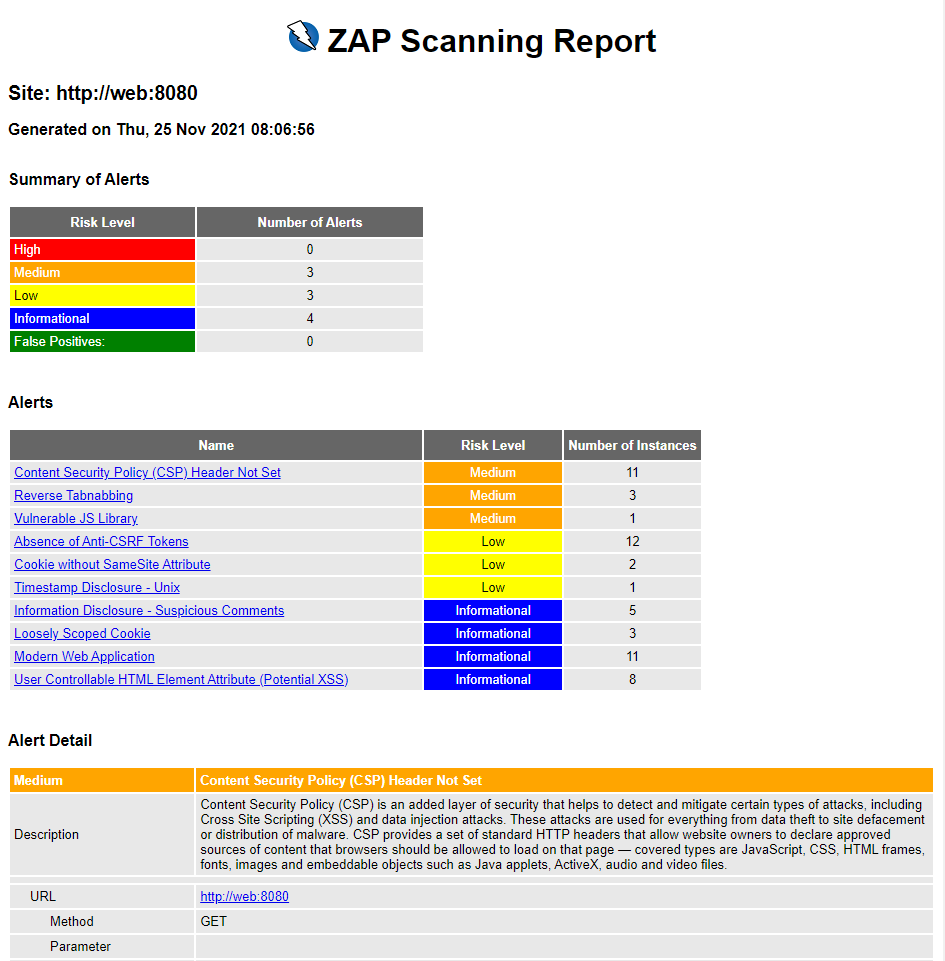
\includegraphics[scale=0.5]{images/zap-report}
    \caption{Bericht nach der Ausführung einer Zap Baseline} \label{fig:baseline}
\end{figure}
